\chapter{Identity and Access Management}
\label{ch:identity-and-access-management}

You should refer to the following resources in additon to the
explanations in these notes:

\begin{itemize}
\item
  \url{https://docs.aws.amazon.com/IAM/latest/UserGuide/introduction.html}
\item
  \url{https://docs.aws.amazon.com/IAM/latest/UserGuide/best-practices.html}
\end{itemize}

\section{Root credentials}\label{root-credentials}

Like most other IT services, use of AWS requires a login. The form that
this takes depends on what method the user accesses the service by:

\begin{description}
\item[AWS console]
is accessed by providing e-mail (tied to AWS account) and password.
\item[AWS CLI/SDK]
is accessed using two similar credentials:

\begin{description}
\item[AWS Access Key ID]
which functions like a username.
\item[Secret key]
which functions like a password, and must be kept secret. As this is
normally not typed often nor from memory, it is longer than most normal
passwords.
\end{description}

Unlike the e-mail and password, an AWS account can have 2 access keys
(active or inactive) at any one time.
\end{description}

Once satisfactory credentials are provided, we can use any AWS services
we want. This is termed our \emph{root credentials}, and is the
equivalent of the \texttt{root} account on UNIX-like OSes and the local
\texttt{Administrator} on Windows OS.

\subsection{Root usage vulnerability}\label{root-usage-vulnerability}

The standard root credentials are easy to use starting off. However,
having a single set of credentials for all-or-nothing access to all
provisioned resources can lead to problems. Consider some of the
following scenarios:

\begin{enumerate}
\def\labelenumi{\arabic{enumi}.}
\item
  A company provisions an AWS account to host a number of different
  services on. Multiple employees need to be able to use and administer
  different AWS resources relevant only to their work function.
\item
  A distributed system is built where certain parts of the system need
  differing levels of access (think least privilage!)
\item
  A contractor or consultant is employed to help with setting up certain
  AWS resources. We don't want them to access all of our production
  data, only test data.
\item
  Some ``users'' will not be people at all, but resources within and
  outside AWS that we need to access AWS resources within our account.
\item
  We wish to log actions done and associate them to individual users.
\end{enumerate}

We need a way to allow more restricted access to specific resources
within an AWS account, essentially an account-within-an-account
scenario.

\section{IAM Users and groups}\label{iam-users-and-groups}

\begin{description}
\item[User:]
each IAM user can be configured for:

\begin{description}
\item[AWS console access]
using a username/password.
\item[AWS CLI/SDK access]
using a set of keys, similar to the root account.
\end{description}
\item[Groups:]
each IAM user can be a member of any number of IAM groups.
\end{description}


\section{Policies}\label{policies}

By default, an IAM user has no permissions to do anything with the AWS
account. Policies are used to grant specific permissions. Policies are
distinct objects that are normally expressed/shown in JSON form. A
policy consists of a number of statements:

\subsection{Policy elements}\label{policy-elements}

Each policy consists of 1 or more statements that each contain the
following elements:

\begin{description}
\item[Sid:]
each statement is identified by its Sid.
\item[Effect:]
is to either allow or deny
\item[Principal:]
is the user (not group!) to which this policy applies.
\item[Action:]
is a list of the actions to control. Allowed actions are listed for each
AWS service.
\item[Resource:]
is the list of resources to apply this policy to, in ARN format.
\item[Condition:]
can limit the applicability of the policy (see later!)
\end{description}

\subsection{Resource and identity-based
policies}\label{resource-and-identity-based-policies}

\begin{description}
\item[Resource-based policies]
are attached to resources (rather than users/groups) and state what
actions a principal is allow to perform on the resource.
\item[Identity-based policies]
are attached to a user or group and state what actions the user/group
can perform on what resources and subject to a number of conditions.
\end{description}

\subsection{Managed vs inline
policies}\label{managed-vs-inline-policies}

Identity-based policies can be either managed or inline:

\begin{description}
\item[Managed policies]
\begin{description}
\item[AWS managed policies]
created and controlled by AWS for many common scenarios.
\item[Customer-managed policies]
created and controlled by the AWS account holder. More precise control.
Written in JSON or with the help of the policy editor.
\end{description}
\item[Inline policies]
are embedded directly with a user/group. Not recommended for
identity-based policies.
\end{description}

Note that all resource-based policies are inline! There are no managed
resource-based policies.

\subsection{Policy evaluation}\label{policy-evaluation}

So far, we can see that multiple different policies may be defined
relating to a resource or principal. shows the evaluation flow used by
AWS. Note that when more complex IAM features are used, this causes
further steps to appear in the process.

\begin{figure}
\centering
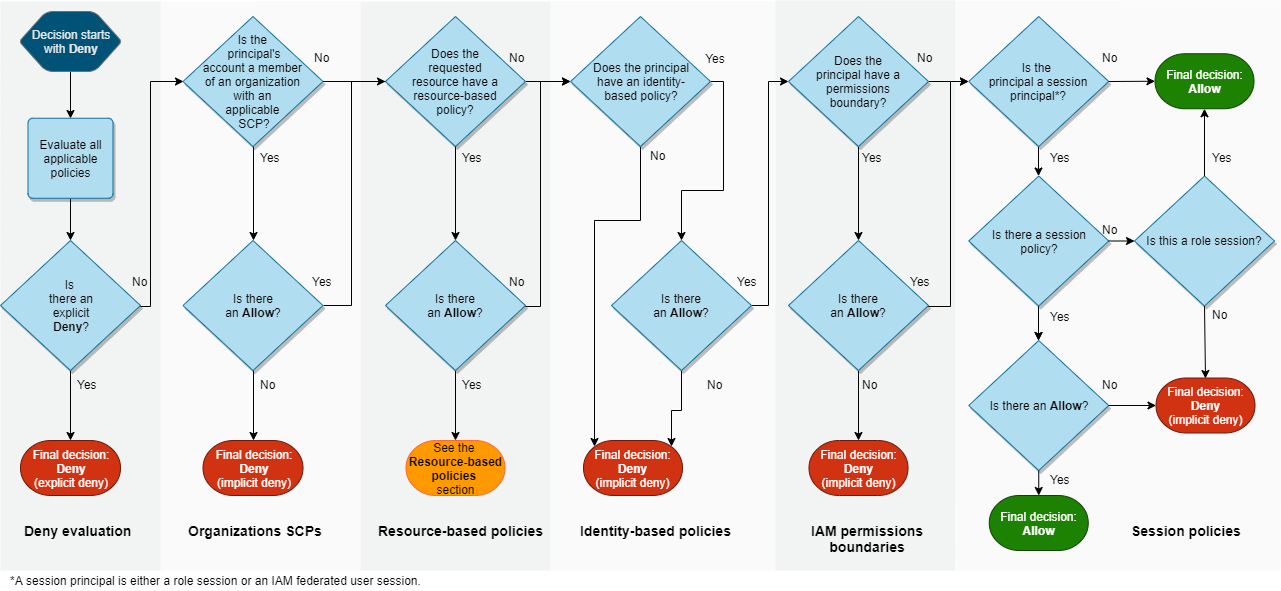
\includegraphics{iam_policy_evaluation}
\caption{Simplified AWS policy evaluation flow (adapted from AWS
documentation, some category steps omitted){}}
\end{figure}
